% Session 2 -- the 1D band, annotated.
% Placement: sec. "Bloch's theorem and the first band structure", after eq. (2.8).
% Rendered by figures/blender/s02f02_cosband.py, labels in figures/overlays/s02f02_cosband.tex.
\begin{aqmfigure}{fig:s02:cosband}{The one-dimensional band $\epsilon_\varphi=-2t\cos\varphi$ of
(2.8), drawn for $t=1$, with the grey tubes showing its local forms. Near the band bottom the
dispersion is an upward parabola, and quasiparticles behave as ordinary electrons with positive
mass. Near the top the curvature has the opposite sign and they behave as holes. Near midband it is
locally linear, which is a first sign of the Dirac physics of Section 2.11. The slope is the group
velocity (2.17) and the curvature is the inverse effective mass (2.18), and both are read from this
one curve. On the right is the resulting density of states (2.16), cut at the top of the drawing,
which diverges at both band edges, at the same points where the group velocity vanishes.}
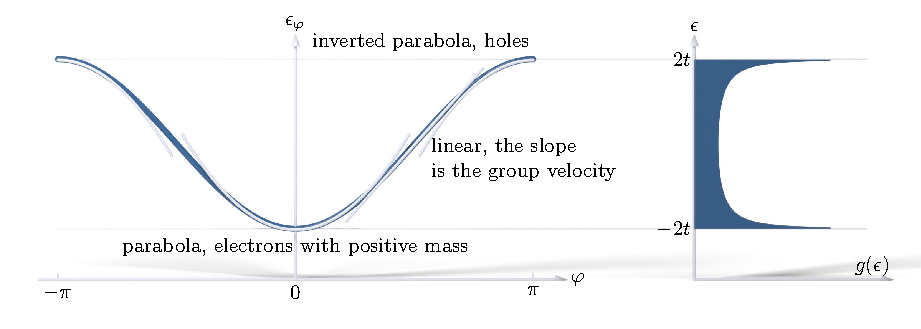
\includegraphics{figures/pdf/s02f02_cosband.pdf}
\end{aqmfigure}
